\documentclass[11pt, a4paper, titlepage, block]{article}
\hyphenpenalty=10000
\begin{document}
	\begin{titlepage}

		\newcommand{\HRule}{\rule{\linewidth}{0.5mm}} % Defines a new command for the horizontal lines, change thickness here

		\center % Center everything on the page

		%----------------------------------------------------------------------------------------
		%  HEADING SECTIONS
		%----------------------------------------------------------------------------------------

		\textsc{\LARGE Universit\`a di Urbino}\\[1.5cm] % Name of your university/college
		\textsc{\Large Informatica Applicata}\\[0.5cm] % Major heading such as course name
		\textsc{\large Programmazione Procedurale e Logica}\\[0.5cm] % Minor heading such as course title

		%----------------------------------------------------------------------------------------
		%  TITLE SECTION
		%----------------------------------------------------------------------------------------


		\HRule \\[0.4cm]
		{ \huge \bfseries Relazione}\\[0.2cm] % Title of your document
		\HRule \\[0.4cm]
		\textsc{\large Progetto per la sessione invernale 2014/2015}
		\\[2cm]
		%----------------------------------------------------------------------------------------
		%  AUTHOR SECTION
		%----------------------------------------------------------------------------------------

		\begin{minipage}{\textwidth}
			\begin{flushleft}
				\emph{Studente:}\\
				Marco \textsc{Tamagno}\\ % Your name
				matricola no: 261985
				\\[1cm]
				\emph{Studente:}\\
				Julian \textsc{Sparber}\\ % Your name
				matricola no: 260492\\
			\end{flushleft}
		\end{minipage}\\[3cm]

		\begin{minipage}{\textwidth}
			\begin{flushright}
				\emph{Professore:} \\
				 Antonio\textsc{Della Selva}\\ % Supervisor`s Name
			\end{flushright}
		\end{minipage}\\[4cm]

		{\today}\\[1cm]


		%----------------------------------------------------------------------------------------
		%  DATE SECTION
		%----------------------------------------------------------------------------------------

	 % Date, change the \today to a set date if you want to be precise
		%----------------------------------------------------------------------------------------
		%  LOGO SECTION
		%----------------------------------------------------------------------------------------
		%\includegraphics{Logo}\\[1cm] % Include a department/university logo - this will require the graphicx package
		%----------------------------------------------------------------------------------------
		\newpage
		\tableofcontents
		\newpage

	\end{titlepage}

	\section{Specifica del Problema}
Creare sfruttando webRTC una simulazione del gioco del pong a 4 giocatori dove gli utenti connessi tramite browser si scambino informazioni tramite peer to peer

	\section{Analisi del Problema}

WebRTC è una tecnologia open source nata il 1º giugno 2011 che consente ai browser di effettuare in tempo reale la videochat. È basata su HTML5 e JavaScript.\\
La sua inclusione nel World Wide Web Consortium (W3C) standard è supportato da Google, Mozilla e Opera.\\
È rilasciato sotto la parziale licenza BSD e il codice si basa su prodotti di Global IP Solutions, azienda che Google ha acquisito nel maggio 2010 per 68 milioni di euro.\\
WebRTC utilizza per l'audio il codec Opus e il codec VP8 per il video e si sta lavorando a migrare il plugin di Google Talk video chat per il quadro webRTC.
\\
STUN è l'acronimo di Session Traversal Utilities for Network Address Translators (NATs): si tratta di un protocollo e di un insieme di funzioni che permettono alle applicazioni in esecuzione su un computer di scoprire la presenza ed i tipi di NAT e firewall che si interpongono tra il computer e la rete pubblica.\\
STUN permette a queste applicazioni di conoscere gli indirizzi IP e le porte con cui il dispositivo NAT li sta rendendo visibili sulla rete pubblica. STUN opera con molti NAT preesistenti e non richiede particolari comportamenti da essi.\\
Come risultato, STUN assicura ad una grande varietà di applicazioni IP (ad esempio, i telefoni VoIP) di lavorare attraverso le varie strutture NAT preesistenti.

Nella specifica originaria in RFC 3489, STUN era l'acronimo di Simple Traversal of User Datagram Protocol (UDP) Through Network Address Translators (NATs), ma nella specifica aggiornata pubblicata come RFC 5389 il titolo è mutato in Session Traversal Utilities for NAT, mantenendo lo stesso acronimo.\\

STUN è un protocollo client-server. Un telefono o un software VoIP può includere un client STUN, che invierà una richiesta ad un server STUN. Il server riporterà al client STUN l'indirizzo IP pubblico e la porta UDP che il dispositivo NAT (es. router) sta associando al client per il traffico entrante nella rete.\\
Le risposte permettono anche al client STUN di determinare che tipo di NAT è in uso.\\
Ci sono tre tipi di NAT che è possibile attraversare tramite STUN: Full Cone, Restricted Cone e Port Restricted Cone.\\
STUN non lavora con il quarto tipo di NAT, detto simmetrico o bidirezionale, questo a causa del fatto che i dati trovati dal server STUN non saranno validi per terze parti, in quanto il NAT bidirezionale non permette a terzi di riusare IP e porte abilitate, differenziando le associazioni a seconda dell'host contattato.\\

Client e server STUN sono utilizzati con protocolli come SIP tramite UDP per il trasferimento di traffico voce/video/testo su Internet.\\
\\

WebRTC tramite un iceserver sfruttato per l autenticazione mette in una comunicazione peertopeer due o piu' browser.\\
Il gioco del pong e' composto da questi elementi:\\
una pallina\\
una racchetta (una per ogni giocatore)\\
una stanza (dove verra' svolta la partita)\\
una rete (dove verranno segnati i gol)\\
\\
Ogni giocatore inviera' a ogni altro giocatore la posizione della propia racchetta.\\
Il giocatore master, in possesso della pallina comunichera' a tutti gli altri giocatori la posizione della pallina.
Ogni giocatore inviera' agli altri giocatori il numero di reti che ha subito.\\
\\
\\
Ogni stanza ospitera' una partita differente.\\
Gli utenti "extra" potranno far da spettatori alla partita.\\

\section{Scelte di Progetto}
	Abbiamo deciso di utilizzare lo stun/turn server reso disponibile da google.

\section{Testing del Programma}
	Screenshots:
\\
\\
All inizio del gioco aspetto l arrico di 4 giocatori..
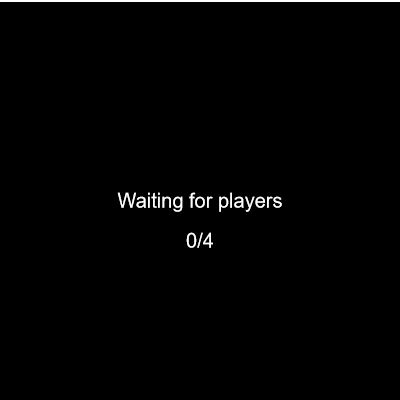
\includegraphics[width=3in,height=3in,viewport=0 0 300 300]{../Screenshots/Capture1.jpg}
\\
\\
Una volta connessi i 4 giocatori il master invia agli altri giocatori la pallina..
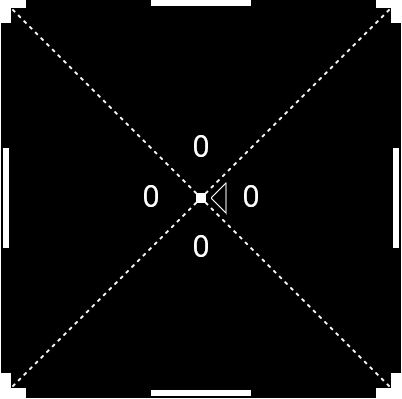
\includegraphics[width=3in,height=3in,viewport=0 0 300 300]{../Screenshots/Capture2.jpg}
\\
\\
E i suoi relativi spostamenti..
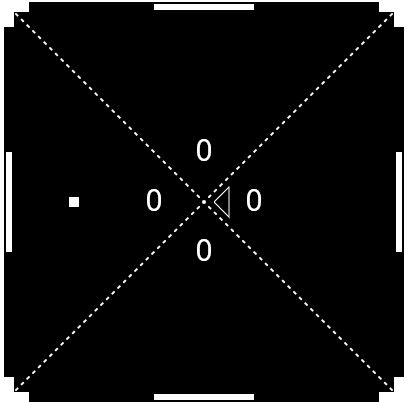
\includegraphics[width=3in,height=3in,viewport=0 0 300 300]{../Screenshots/Capture3.jpg}
\\
\\
Ogni giocatore invia i gol subiti agli altri giocatori..
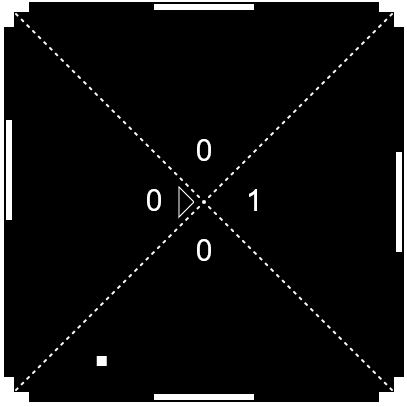
\includegraphics[width=3in,height=3in,viewport=0 0 300 300]{../Screenshots/Capture4.jpg}
	\\	
	\\

\end{document}
